\documentclass[tikz,border=2pt]{standalone}
\pdfmapfile{+cm.map}
\usepackage{pgfplots}
\pgfplotsset{compat=1.18}
\usetikzlibrary{arrows.meta}
\definecolor{ink}{HTML}{202B30}
\definecolor{red}{HTML}{971D2C}
\definecolor{soft}{HTML}{F4E9EB}
\definecolor{gray}{HTML}{51636D}
\definecolor{line}{HTML}{D6DDE0}
\definecolor{pale}{HTML}{F0F3F4}
\begin{document}
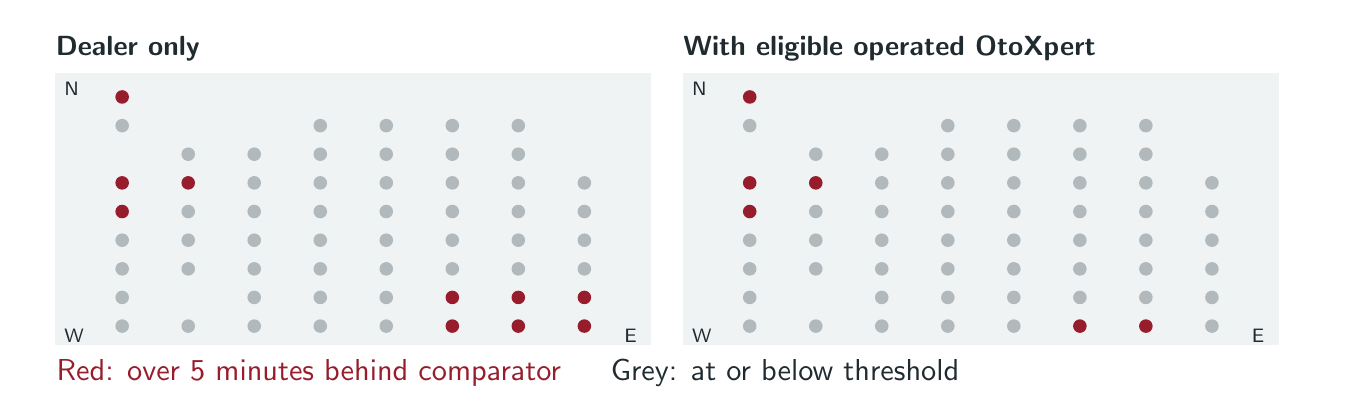
\begin{tikzpicture}[x=1cm,y=1cm,font=\sffamily\fontsize{10.5}{12}\selectfont,text=ink,arr/.style={-{Stealth[length=2mm]},draw=gray,thick}]
\path[use as bounding box] (0,0) rectangle (16.4,4.61);
\node[anchor=west,inner sep=0pt,font=\sffamily\bfseries] at (0.35,4.35) {Dealer only};
\fill[pale] (0.35,0.58) rectangle (7.92,4.03);
\fill[gray!45] (1.200,0.820) circle (2.45pt);\fill[gray!45] (2.039,0.820) circle (2.45pt);\fill[gray!45] (2.877,0.820) circle (2.45pt);\fill[gray!45] (3.716,0.820) circle (2.45pt);\fill[gray!45] (4.554,0.820) circle (2.45pt);\fill[red] (5.393,0.820) circle (2.45pt);\fill[red] (6.231,0.820) circle (2.45pt);\fill[red] (7.070,0.820) circle (2.45pt);\fill[gray!45] (1.200,1.184) circle (2.45pt);\fill[gray!45] (2.877,1.184) circle (2.45pt);\fill[gray!45] (3.716,1.184) circle (2.45pt);\fill[gray!45] (4.554,1.184) circle (2.45pt);\fill[red] (5.393,1.184) circle (2.45pt);\fill[red] (6.231,1.184) circle (2.45pt);\fill[red] (7.070,1.184) circle (2.45pt);\fill[gray!45] (1.200,1.547) circle (2.45pt);\fill[gray!45] (2.039,1.547) circle (2.45pt);\fill[gray!45] (2.877,1.547) circle (2.45pt);\fill[gray!45] (3.716,1.547) circle (2.45pt);\fill[gray!45] (4.554,1.547) circle (2.45pt);\fill[gray!45] (5.393,1.547) circle (2.45pt);\fill[gray!45] (6.231,1.547) circle (2.45pt);\fill[gray!45] (7.070,1.547) circle (2.45pt);\fill[gray!45] (1.200,1.911) circle (2.45pt);\fill[gray!45] (2.039,1.911) circle (2.45pt);\fill[gray!45] (2.877,1.911) circle (2.45pt);\fill[gray!45] (3.716,1.911) circle (2.45pt);\fill[gray!45] (4.554,1.911) circle (2.45pt);\fill[gray!45] (5.393,1.911) circle (2.45pt);\fill[gray!45] (6.231,1.911) circle (2.45pt);\fill[gray!45] (7.070,1.911) circle (2.45pt);\fill[red] (1.200,2.275) circle (2.45pt);\fill[gray!45] (2.039,2.275) circle (2.45pt);\fill[gray!45] (2.877,2.275) circle (2.45pt);\fill[gray!45] (3.716,2.275) circle (2.45pt);\fill[gray!45] (4.554,2.275) circle (2.45pt);\fill[gray!45] (5.393,2.275) circle (2.45pt);\fill[gray!45] (6.231,2.275) circle (2.45pt);\fill[gray!45] (7.070,2.275) circle (2.45pt);\fill[red] (1.200,2.639) circle (2.45pt);\fill[red] (2.039,2.639) circle (2.45pt);\fill[gray!45] (2.877,2.639) circle (2.45pt);\fill[gray!45] (3.716,2.639) circle (2.45pt);\fill[gray!45] (4.554,2.639) circle (2.45pt);\fill[gray!45] (5.393,2.639) circle (2.45pt);\fill[gray!45] (6.231,2.639) circle (2.45pt);\fill[gray!45] (7.070,2.639) circle (2.45pt);\fill[gray!45] (2.039,3.003) circle (2.45pt);\fill[gray!45] (2.877,3.003) circle (2.45pt);\fill[gray!45] (3.716,3.003) circle (2.45pt);\fill[gray!45] (4.554,3.003) circle (2.45pt);\fill[gray!45] (5.393,3.003) circle (2.45pt);\fill[gray!45] (6.231,3.003) circle (2.45pt);\fill[gray!45] (1.200,3.366) circle (2.45pt);\fill[gray!45] (3.716,3.366) circle (2.45pt);\fill[gray!45] (4.554,3.366) circle (2.45pt);\fill[gray!45] (5.393,3.366) circle (2.45pt);\fill[gray!45] (6.231,3.366) circle (2.45pt);\fill[red] (1.200,3.730) circle (2.45pt);\node[anchor=west,inner sep=0pt,font=\sffamily\scriptsize] at (0.45999999999999996,0.7) {W};
\node[anchor=west,inner sep=0pt,font=\sffamily\scriptsize] at (7.569999999999999,0.7) {E};
\node[anchor=west,inner sep=0pt,font=\sffamily\scriptsize] at (0.45999999999999996,3.83) {N};
\node[anchor=west,inner sep=0pt,font=\sffamily\bfseries] at (8.32,4.35) {With eligible operated OtoXpert};
\fill[pale] (8.32,0.58) rectangle (15.89,4.03);
\fill[gray!45] (9.170,0.820) circle (2.45pt);\fill[gray!45] (10.009,0.820) circle (2.45pt);\fill[gray!45] (10.847,0.820) circle (2.45pt);\fill[gray!45] (11.686,0.820) circle (2.45pt);\fill[gray!45] (12.524,0.820) circle (2.45pt);\fill[red] (13.363,0.820) circle (2.45pt);\fill[red] (14.201,0.820) circle (2.45pt);\fill[gray!45] (15.040,0.820) circle (2.45pt);\fill[gray!45] (9.170,1.184) circle (2.45pt);\fill[gray!45] (10.847,1.184) circle (2.45pt);\fill[gray!45] (11.686,1.184) circle (2.45pt);\fill[gray!45] (12.524,1.184) circle (2.45pt);\fill[gray!45] (13.363,1.184) circle (2.45pt);\fill[gray!45] (14.201,1.184) circle (2.45pt);\fill[gray!45] (15.040,1.184) circle (2.45pt);\fill[gray!45] (9.170,1.547) circle (2.45pt);\fill[gray!45] (10.009,1.547) circle (2.45pt);\fill[gray!45] (10.847,1.547) circle (2.45pt);\fill[gray!45] (11.686,1.547) circle (2.45pt);\fill[gray!45] (12.524,1.547) circle (2.45pt);\fill[gray!45] (13.363,1.547) circle (2.45pt);\fill[gray!45] (14.201,1.547) circle (2.45pt);\fill[gray!45] (15.040,1.547) circle (2.45pt);\fill[gray!45] (9.170,1.911) circle (2.45pt);\fill[gray!45] (10.009,1.911) circle (2.45pt);\fill[gray!45] (10.847,1.911) circle (2.45pt);\fill[gray!45] (11.686,1.911) circle (2.45pt);\fill[gray!45] (12.524,1.911) circle (2.45pt);\fill[gray!45] (13.363,1.911) circle (2.45pt);\fill[gray!45] (14.201,1.911) circle (2.45pt);\fill[gray!45] (15.040,1.911) circle (2.45pt);\fill[red] (9.170,2.275) circle (2.45pt);\fill[gray!45] (10.009,2.275) circle (2.45pt);\fill[gray!45] (10.847,2.275) circle (2.45pt);\fill[gray!45] (11.686,2.275) circle (2.45pt);\fill[gray!45] (12.524,2.275) circle (2.45pt);\fill[gray!45] (13.363,2.275) circle (2.45pt);\fill[gray!45] (14.201,2.275) circle (2.45pt);\fill[gray!45] (15.040,2.275) circle (2.45pt);\fill[red] (9.170,2.639) circle (2.45pt);\fill[red] (10.009,2.639) circle (2.45pt);\fill[gray!45] (10.847,2.639) circle (2.45pt);\fill[gray!45] (11.686,2.639) circle (2.45pt);\fill[gray!45] (12.524,2.639) circle (2.45pt);\fill[gray!45] (13.363,2.639) circle (2.45pt);\fill[gray!45] (14.201,2.639) circle (2.45pt);\fill[gray!45] (15.040,2.639) circle (2.45pt);\fill[gray!45] (10.009,3.003) circle (2.45pt);\fill[gray!45] (10.847,3.003) circle (2.45pt);\fill[gray!45] (11.686,3.003) circle (2.45pt);\fill[gray!45] (12.524,3.003) circle (2.45pt);\fill[gray!45] (13.363,3.003) circle (2.45pt);\fill[gray!45] (14.201,3.003) circle (2.45pt);\fill[gray!45] (9.170,3.366) circle (2.45pt);\fill[gray!45] (11.686,3.366) circle (2.45pt);\fill[gray!45] (12.524,3.366) circle (2.45pt);\fill[gray!45] (13.363,3.366) circle (2.45pt);\fill[gray!45] (14.201,3.366) circle (2.45pt);\fill[red] (9.170,3.730) circle (2.45pt);\node[anchor=west,inner sep=0pt,font=\sffamily\scriptsize] at (8.43,0.7) {W};
\node[anchor=west,inner sep=0pt,font=\sffamily\scriptsize] at (15.54,0.7) {E};
\node[anchor=west,inner sep=0pt,font=\sffamily\scriptsize] at (8.43,3.83) {N};
\node[anchor=west,inner sep=0pt,text=red] at (0.36,0.23) {Red: over 5 minutes behind comparator};
\node[anchor=west,inner sep=0pt,] at (7.4,0.23) {Grey: at or below threshold};
\end{tikzpicture}\end{document}